\documentclass{beamer}

\usepackage[utf8]{inputenc}
\usepackage[czech]{babel}
\usepackage[normalem]{ulem}

\usetheme{Blacko}

\setcounter{tocdepth}{2}  % hide subsubsections and lower
  
\setbeamercovered{%
  again covered={\opaqueness<1->{15}}}

\title{\texttt{\LARGE Dvoukanálový USB osciloskop}}
\subtitle{ Obhajoba DMP }
\author{ Adam Verner\footnote{\texttt{vernead15@sps-prosek.cz}}}

\begin{document}

\begin{frame}
	\maketitle \\
\end{frame}
	
\section{Cíle}

	\begin{frame}{Goals}
		\begin{itemize}
			\item Hardware
			\item Firmware
			\item PC App
			\item Ecosystem
		\end{itemize}
	\end{frame}

\section{Hardware}

%	\begin{frame}{FPGA}
%		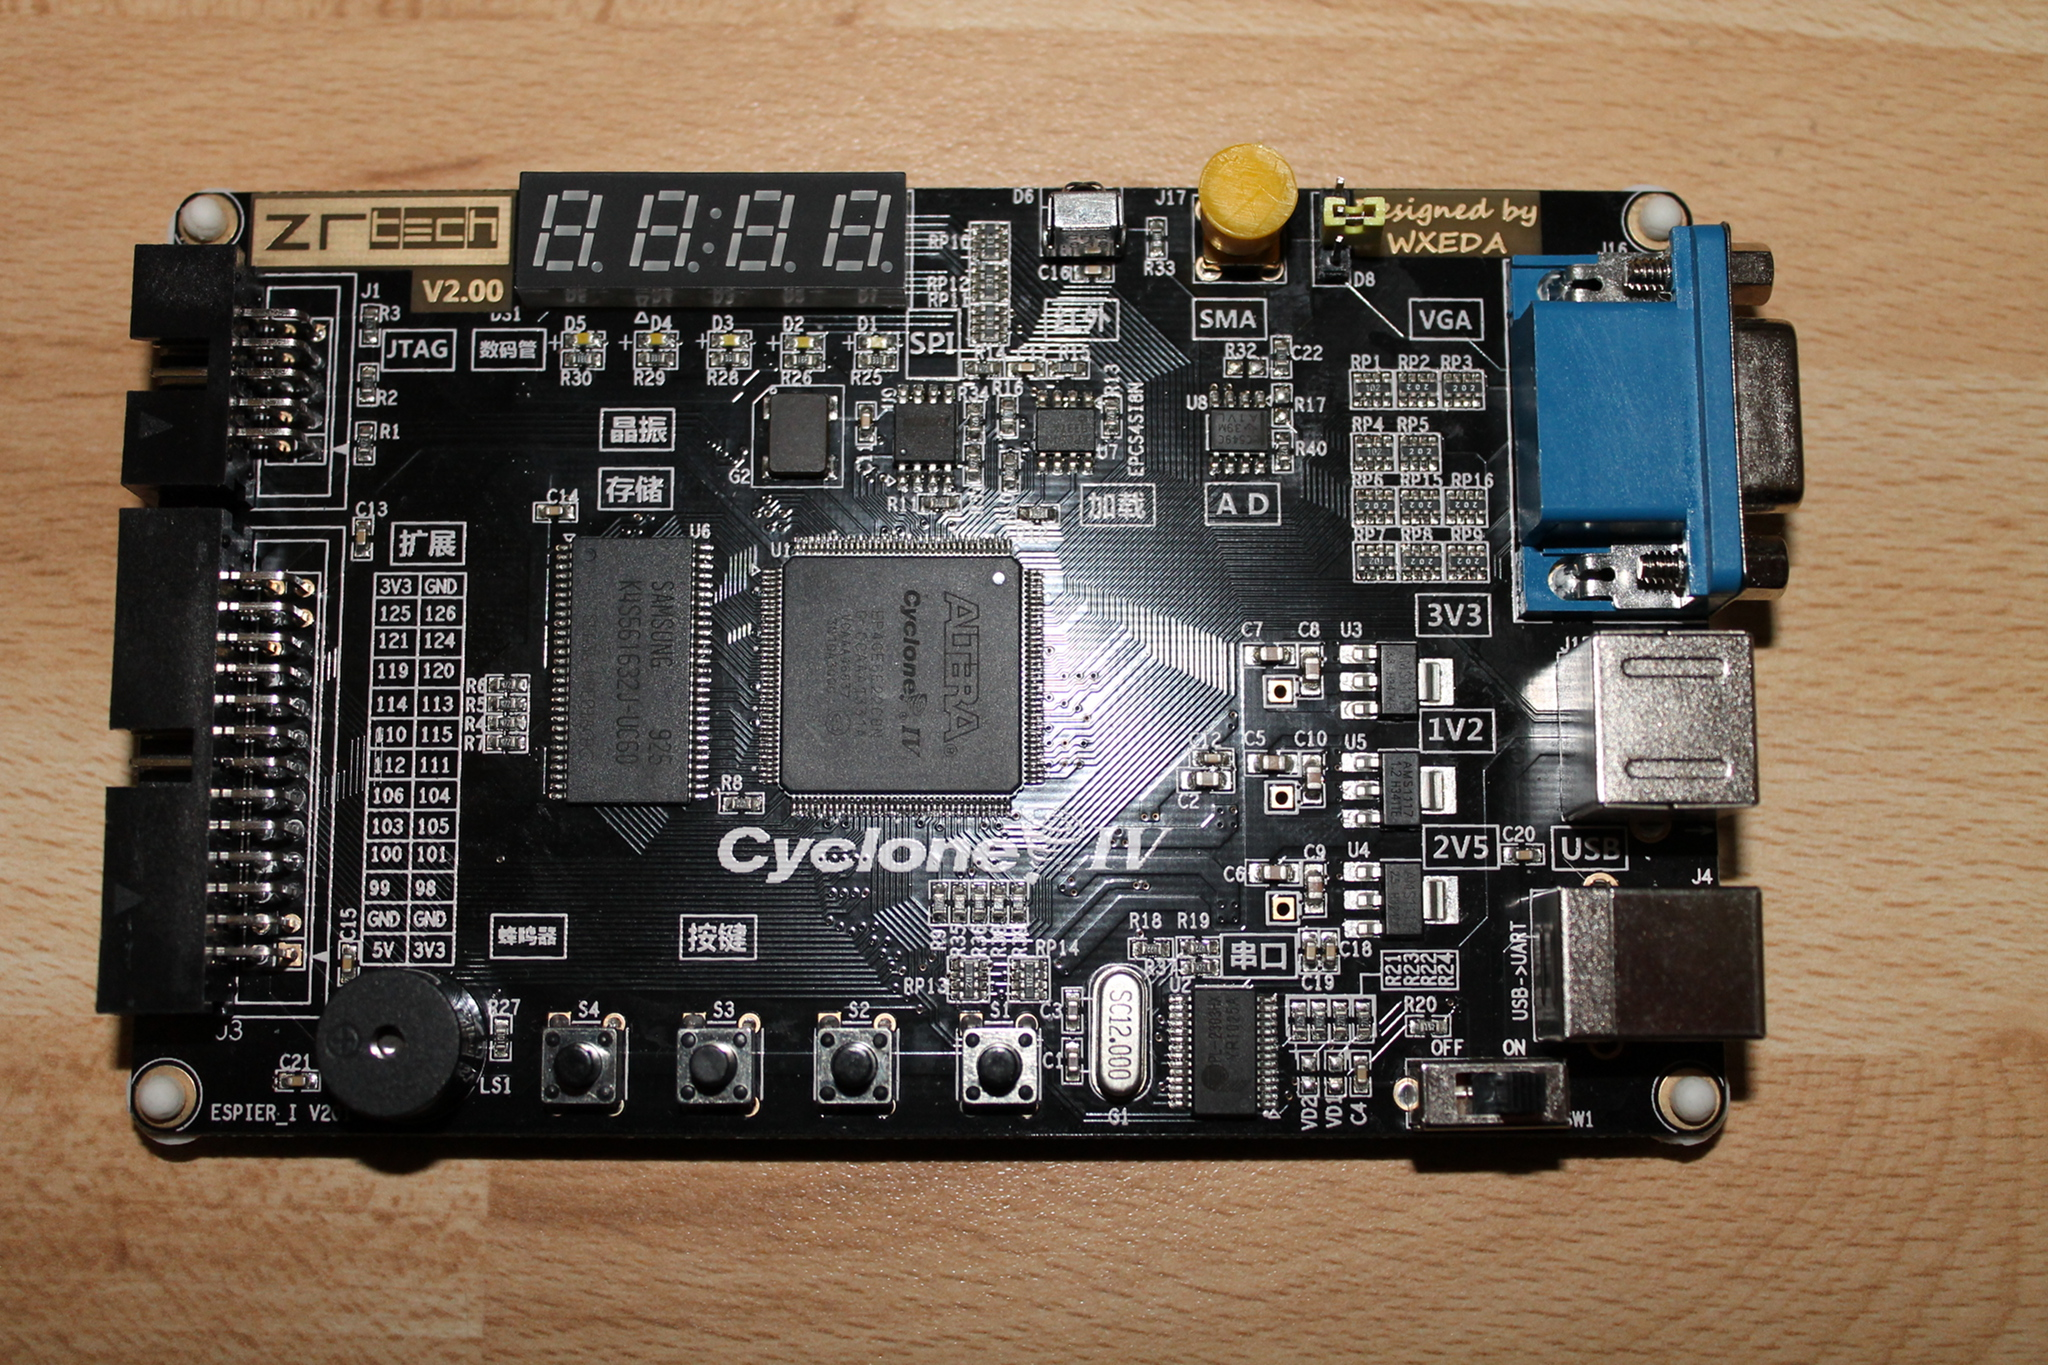
\includegraphics[width=\paperwidth]{ZRtech_board.jpg}
%	\end{frame}

%	
%	\begin{frame}{ADC}
%		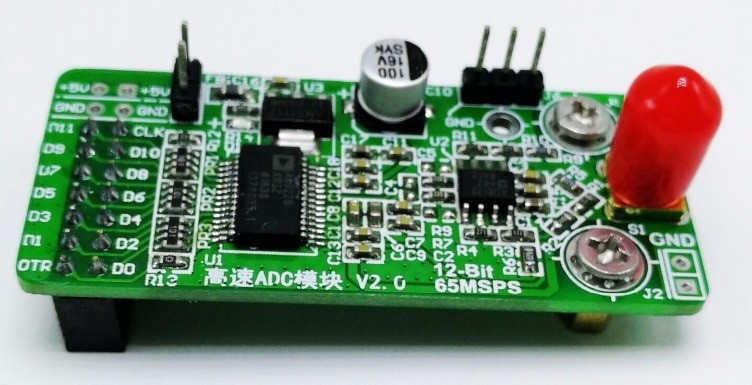
\includegraphics[width=\paperwidth]{adc_board.jpg}
%	\end{frame}

	\begin{frame}{Hardware topology}
		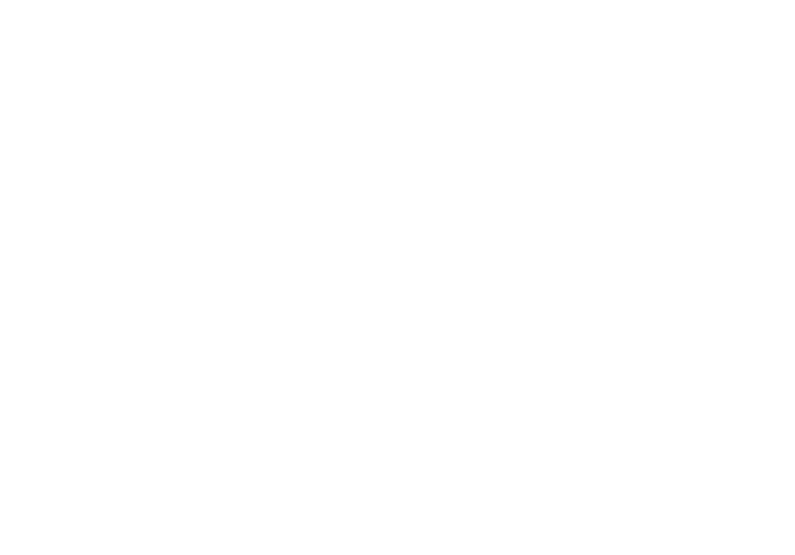
\includegraphics[width=0.9\paperwidth]{Topology.png}
	\end{frame}

	\begin{frame}{Properties}
		\begin{itemize}
			\item 50 MSPS
			\item $<$0.15 sec refresh
			\item 12bit precision $\approx$ 2.44 mV step
			\item 100Mb sample memmory
			\item upto 460,800 baud
		\end{itemize}
	\end{frame}


\section{Firmware}
	\begin{frame}{Firmware}
		\begin{itemize}
			\item system
		\end{itemize}
	\end{frame}

	\begin{frame}
		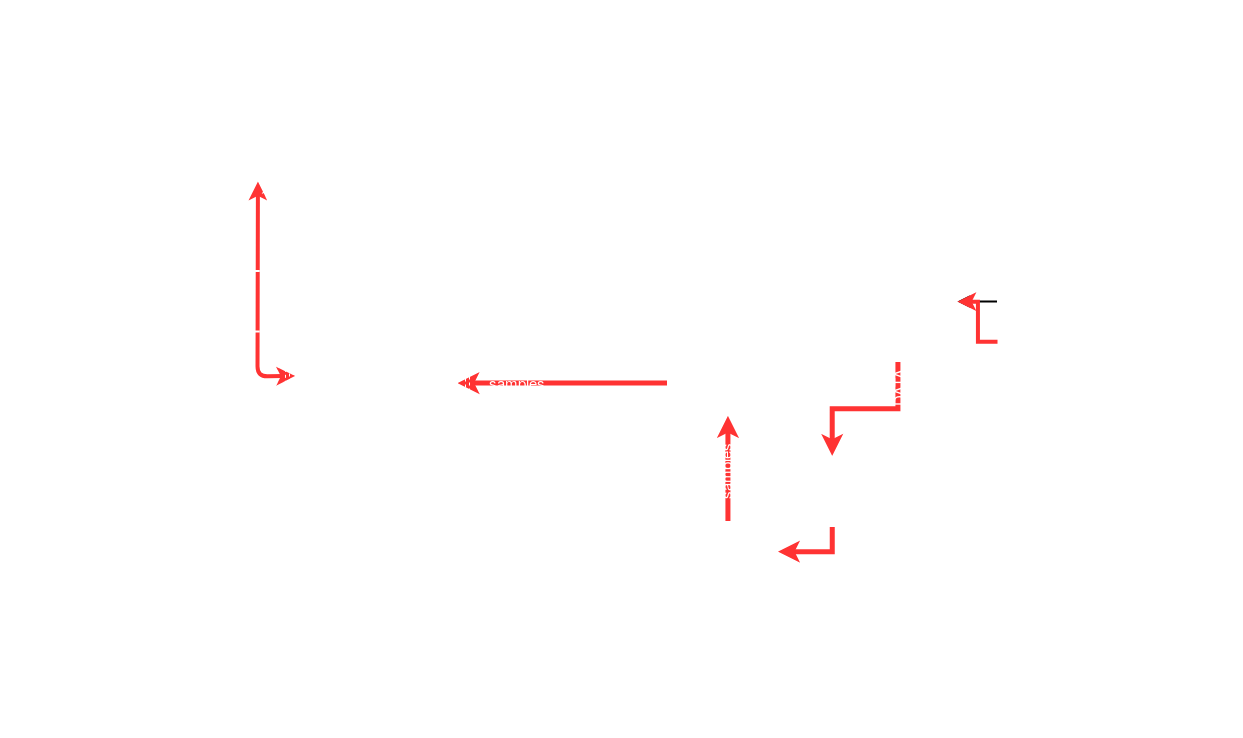
\includegraphics[width=1\paperwidth]{Firmware.png}
	\end{frame}

	\begin{frame}{Firmware}
		\begin{itemize}
			\item system
			\item protocol
			\item tests
		\end{itemize}
	\end{frame}

\section{PC APP}
	\begin{frame}{What can we do}
		\begin{itemize}
			\item Waveform display
			\item Device configration
			\item Data analysis \& exportation
			\item tests
		\end{itemize}
	\end{frame}


	\begin{frame}{Structure}
		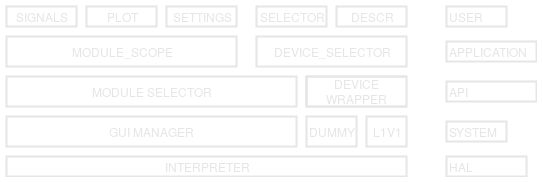
\includegraphics[width=0.9\paperwidth]{SWlayers.png}
	\end{frame}



\begin{frame}{}
	\Huge Děkuji za pozornost.
\end{frame}
\end{document}
\endinput

